\chapter{Asking Millionaires How They Got Rich! (New York City)}

This chapter is not a blackboard lecture in the ordinary sense. We are given no formal derivation on the screen, and yet the lecture has a definite mathematical spine. The host proceeds by repeated interrogation: How much did you make? What was the turning point? What rule mattered? From those recurring questions we recover a structure of cash floors, return thresholds, compounding horizons, sales volume, and role choice under constraint. We keep the order of the interviews, because the lesson is cumulative. Each speaker adds a new piece to the same problem: how wealth is accumulated, preserved, scaled, and interpreted.

\section{New York as a Field Laboratory}

The lecture opens with a cold montage of outcomes: large annual numbers, personal maxims, and recognizable entrepreneurs. We should read that opening as a promise rather than as the lecture proper. It tells us the destination before it tells us the method.

The method comes a few moments later. New York City is presented as a dense environment of millionaires, and the lecture takes the city itself as a laboratory. The host will move through that environment asking nearly the same sequence of questions each time. This is important. The lecture does not argue from a single theory downward; it argues by repeated comparison across cases. The same numerical prompts return, and the differences in answer begin to matter more than the numbers by themselves.

That repeated protocol is already a kind of notation. We ask about scale, then origin, then mechanism, then transfer. In these notes we shall preserve that order.

\section{Wall Street, Attrition, and the First Resource}

The first full case begins with a sharp quantitative hook: the speaker's best month on Wall Street was about \(\$80{,}000\). But the lecture refuses to leave that number isolated. It immediately places it inside a harsh environment. Wall Street is described as a beast, savage, full of rapid attrition: look left, look right, and many of those people will soon be gone.

That is the lecture's first serious move. Income appears first, but environment appears second. Wealth is not treated as a static prize; it is treated as survival inside a selective machine. The same speaker then adds two further constraints: he became a millionaire only in his forties, and he had been broke many times before. The lecture thereby blocks an easy fantasy of immediate ascent.

\begin{definition}
For later use we define the period surplus by
\begin{equation}
S_t = I_t - E_t,
\end{equation}
where \(I_t\) is inflow over a period and \(E_t\) is expenditure over that same period. This is not a spoken formula from the lecture, but it is the smallest clean mathematical reconstruction of the speaker's claim that accumulation fails when resources are drained away.
\end{definition}

The same interview then turns from competition to discipline. Most people, we are told, cannot say no to themselves; the result is not merely moral weakness but resource depletion. To make that precise we may separate expenditure into what is necessary and what leaks away through undisciplined use:
\begin{equation}
E_t = E_{\text{necessary},t} + E_{\text{leakage},t},
\end{equation}
so that the effective surplus becomes
\begin{equation}
S_{\text{net},t} = I_t - E_{\text{necessary},t} - E_{\text{leakage},t}.
\end{equation}

The lecture's language here is deliberately vivid. ``Your number one resource is your energy.'' We should not literalize that into physics. The point is economic. Energy is the name the speaker gives to deployable attention, discipline, and effort. If that resource is dissipated, then even a large inflow fails to convert into durable accumulation.

\subsection{Question \& Answer}

\paragraph{Question.} What separates those who build wealth from those who drain their own resources?

\paragraph{Answer.} In the first interview, the answer is not a secret asset class or a hidden market. It is discipline interpreted as a conservation law for the self. The speaker's examples are concrete and behavioral, but the mechanism is simple: if leakage rises, surplus falls; if surplus falls, accumulation stalls. In that sense the lecture begins with a negative theorem. Wealth does not first fail because returns are too small. It fails because the system leaks before returns can matter.

\begin{remark}
The lecture later uses phrases such as ``money is a frequency'' and ``money magnet.'' We keep those as rhetoric, not as literal mathematical objects. Their serious content lies in attention, habit, and disciplined alignment, not in any claimed physical law.
\end{remark}

The host then recaps the point in plain language: if we cannot take care of ourselves, we will not take care of our finances. That recap is structurally important. It marks the first interview not as a self-contained anecdote, but as the first term in a growing sequence.

\section{White Space, Long Horizons, and the \(30\%\) Rule}

The second case moves into a different industry altogether: the acai bowl smoothie franchise business. The lecture does this on purpose. It widens the sample. We are no longer allowed to think that the first lesson belonged only to Wall Street. The new speaker reports entrepreneurial activity from childhood onward, then reveals a turn that matters: he began on Wall Street, saw white space in food and beverage, and moved into that gap.

This is the first place where the lecture gives us a clear operational split between two time scales. When it comes to operating businesses, we are told to think very long-term. When it comes to Wall Street-style investing in stocks, bonds, companies, or crypto, the recommendation becomes shorter-term and more tactical.

A useful reconstruction is to define a target return \(r_{\text{target}}\) and exit when that target is reached:
\begin{equation}
r_{\text{target}} \approx 0.30,
\qquad
\frac{P_t - P_0}{P_0} \ge r_{\text{target}}
\Longrightarrow
\text{sell}.
\end{equation}
The exact spoken phrasing in the transcript is imperfect, but the intended rule is clear enough: set a benchmark and do not confuse discipline with endless optimism.

\paragraph{Worked example.} If we buy at price \(P_0\), then the benchmark exit price is
\begin{align}
P^\star &= (1+r_{\text{target}})P_0 \\
&= 1.3\,P_0.
\end{align}
Thus if \(P_0=\$100\), the target is \(P^\star=\$130\). The example is editorial, but it makes the lecture's rule precise: the decision is tied to a benchmark, not to the slogan that everything goes ``to the moon.''

\subsection{Question \& Answer}

\paragraph{Question.} When do we stay in for the long term, and when do we take gains and exit?

\paragraph{Answer.} The lecture's answer is a horizon split. Business-building belongs to the long horizon because it is an operating game of product, expansion, and market occupation. Public-market and speculative positions are treated more tactically: define a return objective, and leave when the benchmark is met. The goal is not perfect top-ticking. The goal is to avoid the greater-fool logic in which every gain is consumed by the fantasy of an even larger gain.

This interview then adds another caution. Betting on oneself can be correct, but it is not a universal command. Some people need the structure of working within an existing organization. The lecture therefore interrupts its own entrepreneurial romance. Autonomy is valuable, but only for the kind of person who can use it well.

\section{Betting on Yourself Without Making It a Universal Law}

The second interview contains a subtle corrective that matters for the whole chapter. The speaker names the best financial decision of his career: he bet on himself. But when the host asks how important it is to go all in, the answer becomes more careful. It is not the best choice for everybody.

We should pause over that. A lesser lecture would have taken ``bet on yourself'' and turned it into a slogan. This lecture instead inserts a type distinction. Some people need external structure; some need self-authored path. The mechanism of wealth therefore depends not only on markets and discipline, but on fit between person and institutional form.

That distinction prepares the next movement. The host recaps the acai interview not by repeating smoothie details, but by drawing out the general lesson: even a business that sounds unusual can produce multimillion-dollar scale if it occupies a real opportunity. This clears the stage for the most quantitative case in the lecture.

\section{Real Estate: Cash Floors, Compounding, and Staying in the Game}

The Ryan Serhant interview begins, again, with a large number. In 2021, he reports, he made \(\$22\) million. But just as before, the lecture does not permit the number to stand alone. It immediately turns to advice: scared money does not make money, and investment must be thought of over the long term. Warren Buffett is invoked not for prestige, but for the structure of compounding.

A cautious mathematical rendering begins with a general wealth update:
\begin{align}
W_{t+1} &= W_t + S_t + R_t, \\
R_t &= rW_t.
\end{align}
Here \(W_t\) is accumulated wealth, \(S_t\) is new surplus from the period, and \(R_t\) is return generated by already invested wealth. In the special case of pure reinvestment with no new injections or withdrawals, we obtain
\begin{align}
W_{t+1} &= W_t + rW_t \\
&= (1+r)W_t,
\end{align}
and therefore by iteration
\begin{equation}
W_t = W_0(1+r)^t.
\end{equation}

This is not a board equation from the lecture, but it is the cleanest standard reconstruction of the interview's point: not tomorrow, but over the lifespan. The speaker's rhetoric of \(10\times\), \(20\times\), \(100\times\) returns should be read in that light. The strict mathematical content is multiplicative growth over time, not an immediate guarantee of extreme outcomes.

The lecture then pivots sharply from scale back to constraint. Before real estate, the speaker had moved to New York in 2006 to do theater and ran out of money. The problem became brutally simple. Which option would keep him in the city? Bartending, waiting tables, temp work, school, or a real-estate license? At that point the lecture introduces, in substance, a cash floor:
\begin{definition}
We call
\begin{equation}
C_{\min} \approx \$2{,}000/\text{month}
\end{equation}
the cash floor: the minimum inflow needed to remain in the game.
\end{definition}
Any option that fails the inequality
\begin{equation}
I_{\text{option}} \ge C_{\min}
\end{equation}
cannot preserve the life one is trying to maintain.

\subsection{Question \& Answer}

\paragraph{Question.} How do we survive long enough for compounding to matter?

\paragraph{Answer.} The lecture's answer is not abstract patience. It is the identification of a floor below which the whole project collapses. Before we can speak about compounding, we must stay solvent. Before we can stay solvent, we must choose a path that clears the monthly threshold. Only then does time become useful. The real-estate license is therefore not introduced as a dream at first; it is introduced as the option that keeps the system alive.

\begin{figure}
\centering
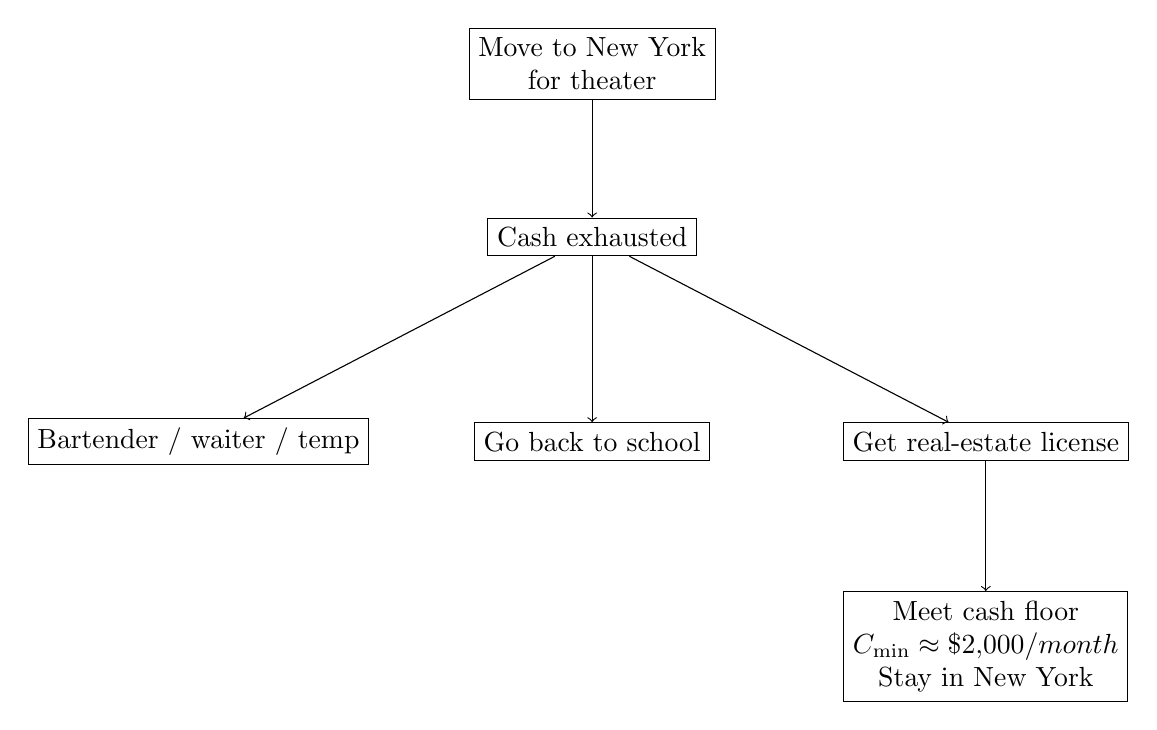
\begin{tikzpicture}[x=1cm,y=1cm]
\node[draw, rectangle, align=center] (start) at (0,0) {Move to New York\\for theater};
\node[draw, rectangle, align=center] (cash) at (0,-2.2) {Cash exhausted};
\node[draw, rectangle, align=center] (bar) at (-5,-4.8) {Bartender / waiter / temp};
\node[draw, rectangle, align=center] (school) at (0,-4.8) {Go back to school};
\node[draw, rectangle, align=center] (license) at (5,-4.8) {Get real-estate license};
\node[draw, rectangle, align=center] (stay) at (5,-7.4) {Meet cash floor\\$C_{\min}\approx \$2{,}000/\text{month}$\\Stay in New York};
\draw[->] (start) -- (cash);
\draw[->] (cash) -- (bar);
\draw[->] (cash) -- (school);
\draw[->] (cash) -- (license);
\draw[->] (license) -- (stay);
\end{tikzpicture}
\end{figure}

\paragraph{Schematic reconstruction.} This diagram is not a redraw of a lecture frame. It is a compact transcription of the decision structure stated aloud: once the speaker's money was gone, the problem became a branching choice under a fixed monthly requirement.

The lecture adds one more layer of timing. He began in real estate on the day Lehman Brothers filed for bankruptcy. That detail matters because it sharpens the point already made: entry into a field need not coincide with easy conditions. Often it coincides with stress, and the survival floor becomes more important precisely when the surrounding environment is unstable.

\section{Niches, Endurance, Sales Volume, and the Value of Time}

The Ryan Serhant interview does not stop at survival. Having established the floor, it climbs back toward scale. The first lesson offered to a newcomer in 2024 is ``riches in niches.'' This is immediately paired with endurance. People move from niche to niche, interpret difficulty as a brick wall, and leave too soon. The lecture's correction is surgical: most of what looks like a wall is only a speed bump.

At this stage it becomes important to separate different kinds of number. The lecture is full of large quantities, but they do not all refer to the same object.

\paragraph{Scale ladder.}
\begin{itemize}
\item Best Wall Street month: \(Y_{\text{best month}} \approx \$80{,}000\).
\item Acai-franchise business output: \(Y_{\text{business,year}} \gtrsim \$20{,}000{,}000\).
\item Ryan Serhant yearly earnings claim: \(Y_{\text{year}} = \$22{,}000{,}000\).
\item Real-estate annual sales volume: \(V_{\text{annual sales}} \approx 4.5\times 10^{9}\).
\item Mercedes-Benz Miami sellout: \(V_{\text{project}} \approx 1.4\times 10^{9}\).
\item Largest single residential sale mentioned: \(V_{\text{single sale}} \approx 195\times 10^{6}\).
\end{itemize}

We should be careful here. Sales volume is not personal income. Asset price is not take-home pay. Project sellout value is not the same as yearly earnings. The lecture invites awe, but the notes should preserve category distinctions.

The interview then turns to billionaires. The claimed lesson is not that they spend constantly, nor that they hoard constantly, but that they understand the value of a dollar and, above all, the value of time. They spend when it makes sense and become cheap when it makes sense. The restaurant anecdote is not about food. It is about the compression of decision time.

The final piece of the Serhant block is direct: learn how to sell. Sales is presented as the master skill of the new economy, especially against the older script of debt, credentialing, a fixed job, and a prepackaged life course. Whether or not we accept that diagnosis in full, the lecture uses it as a general mechanism: sales converts effort into inflow, and multiple inflow streams widen the space of action.

\section{Gary Vee and the Economics of Role Fit}

The final interview changes register. We leave case-specific operating rules and enter a more temperamental domain. Gary Vee's first advice to his younger self is to trust intuition and to fix the inability to be candid with loved ones in work. The point is not mystical inwardness. It is that misalignment between inner judgment and external action can poison decision making even in a highly driven person.

The scaling discussion is equally harsh. Entrepreneurship is described not as a glamorous ascent but as repeated loss interrupted by occasional wins. We may translate the spirit of that claim without pretending there is a precise formula behind it: the system is stochastic, painful, and intolerant of entitlement. Patience and the capacity to absorb repeated blows are treated as structural, not ornamental.

\subsection{Question \& Answer}

\paragraph{Question.} Do we need to be number one?

\paragraph{Answer.} The lecture's answer is no. Not everyone is built to be the founder, the sole principal, or the visible apex. Gary Vee reframes the hierarchy by pointing to the enormous rewards available to elite operators inside gigantic firms. The point is not a verified statistic but an ordering claim: there exist roles below the top title whose payoff exceeds that of nearly all nominal number ones. Once again the lecture returns to fit. The question is not simply, ``How high can we rank?'' It is, ``What role are we actually built to sustain well?''

That answer retroactively clarifies the whole chapter. The Wall Street speaker emphasized discipline. The acai entrepreneur emphasized white space and horizon choice. Ryan Serhant emphasized survival floors, compounding time, specialization, and sales. Gary Vee adds the final condition: even if the opportunity is real, even if the numbers are large, the path must match the structure of the person walking it.

\section{Summary}

The lecture teaches wealth as a sequence of constraints and transformations rather than as a single doctrine. First we must stop leakage and create surplus. Then we must distinguish long operating horizons from shorter trading horizons. Then we must survive the monthly floor that keeps us in the game long enough for compounding to matter. After that come specialization, endurance, sales, and the valuation of time. The final correction is the most important: scale by itself does not tell us what role to choose. We are not only solving for larger numbers. We are solving for a durable fit between person, horizon, market, and method.